\documentclass[journal=jcisd,manuscript=article]{achemso}
% For JCIM / J. Chem. Inf. Model. style; can be changed to other templates
\usepackage{graphicx,booktabs,amsmath,amssymb}
\usepackage[colorlinks=true,citecolor=blue,linkcolor=black]{hyperref}
\usepackage{multirow,array}
\usepackage[utf8]{inputenc}

\title{Physical Opportunity Site Utilization as a Missing Dimension\\
       in Structure-Based 3D Molecular Generation}

\author{Author 1}
\affiliation{Institution}
\author{Author 2}
\affiliation{Institution}

\abbreviations{SBDD,ESField,POSU,SBR,SQD,HEW,SW,HC}

\begin{document}

\maketitle

\begin{abstract}
% ===== TEMPLATE — replace placeholder values with final experiment results =====
Although recent structure-based 3D molecular generators learn rich geometric
regularities from protein-ligand complexes, global plausibility does not guarantee
local physicochemical opportunity utilization. A generated ligand may be chemically
valid, dockable, and geometrically plausible, yet fail to replace displaceable waters,
preserve conserved waters, or fill hydrophobic cavities with compatible atoms.
%
We formalize this gap by introducing Physical Opportunity Site Utilization
(POSU), a rule-based metric that quantifies how well a generated ligand exploits
water- and cavity-derived opportunity sites without relying on any learned model.
Across a test set of 10 pockets, we find that 70\% of pockets exhibit sub-median
direct HEW occupancy at baseline (Site-Blindness Rate), and that HEW occupancy
is uncorrelated with Vina docking score across successful cases
(Spearman $\rho = -0.09$, $p = 0.68$),
confirming that docking score does not substitute for site-level evaluation.
%
To improve HEW occupancy, we introduce ESField, which converts offline-detected
site maps (displaceable high-energy water, conserved stable water, and hydrophobic
cavity sites) into a learned atom-site compatibility potential for inference-time
two-stage generation guidance. Importantly, we construct training pairs to overcome
a fundamental label scarcity problem: co-crystallized ligands seldom occupy water
positions, providing zero positive examples for water displacement. We resolve
this via water-displacement positive pair construction, enabling the potential
to learn that displaceable waters \emph{can} be productively targeted.
%
Under ESField guidance, HEW occupancy improves from 0\% to 15.1\%
(7/10 pockets achieve occupancy, paired $t$-test, $p < 0.01$),
with the gain concentrated on high-energy water replacement sites.
Molecular quality metrics---QED (0.39), molecular diversity
(+27--45\% Vendi score), and Vina docking score---are maintained within
acceptable bounds, and the trade-off between site specificity and molecular
quality is tunable through guidance parameters. Ablation with shuffled site
types and random site coordinates confirms that the improvement depends on
correct physicochemical site identity.
%
These results establish that physical opportunity site utilization is a measurable
and optimizable dimension missing from current evaluation practice, and that
inference-time site-aware guidance can address it without requiring retraining of
the base generator.
\end{abstract}

%---------------------------------------------------------------------
\section{Introduction}
%---------------------------------------------------------------------

Structure-based drug design (SBDD) has been transformed by deep generative models
that produce 3D molecular structures conditioned on protein binding pockets~\cite{RN1,RN2,RN3}.
Methods including TargetDiff~\cite{RN1}, DiffSBDD~\cite{RN2}, DecompDiff~\cite{RN3},
and DrugFlow~\cite{RN4} demonstrate that diffusion and flow-matching models can generate
chemically valid molecules whose predicted binding poses are competitive with docking-based
approaches.

Despite these advances, current SBDD generators share a common limitation: they
treat the binding pocket as a largely homogeneous geometric environment, learning
statistical co-occurrence patterns between protein atoms and ligand atoms. While
this enables the generation of globally plausible molecules, it does not guarantee
that generated ligands explicitly exploit \emph{local physicochemical opportunity
sites}---displaceable high-energy water molecules, conserved structural waters that
should be preserved or engaged via hydrogen bonds, and hydrophobic cavities that
demand complementary non-polar chemistry~\cite{RN5,RN6,RN7}.

The importance of explicit water handling in drug design is well established.
Water molecules in protein binding sites are not passive bystanders: their
displacement or retention can contribute 1--3 kcal/mol to binding free energy,
comparable to a strong hydrogen bond~\cite{RN8,RN9}. Computational tools such
as WaterMap~\cite{RN10}, GCMC simulations~\cite{RN11}, and 3D-RISM~\cite{RN12}
quantify water thermodynamics, but these methods operate as standalone analyses
and have not been integrated into the molecular generation process itself.

We argue that \emph{local physical opportunity site utilization} constitutes a
missing evaluation and optimization dimension in current 3D molecular generation.
To support this claim, we pose and answer four sequential questions:

\begin{enumerate}
    \item \textbf{Gap existence:} Do globally plausible generated molecules
          systematically under-utilize local opportunity sites?
    \item \textbf{Site meaningfulness:} Are the detected sites physically
          meaningful, or are they merely arbitrary spatial anchors?
    \item \textbf{Method effectiveness:} Can inference-time guidance improve
          site utilization without retraining the base generator?
    \item \textbf{Quality preservation:} Does improved site utilization come
          at acceptable cost to molecular quality?
\end{enumerate}

To address the first question, we introduce \textbf{Physical Opportunity Site
Utilization (POSU)}, a rule-based composite metric that quantifies, per site type,
how well a generated ligand interacts with each physical opportunity site. POSU
uses only geometric distances and hard-coded chemical compatibility rules; it
contains no learned parameters and is fully reproducible from an SDF file and
a site map JSON. Using POSU, we define the \textbf{Site-Blindness Rate (SBR)}:
the proportion of globally plausible molecules that exhibit sub-median POSU,
quantifying the disconnect between traditional quality and local site utilization.

For the second question, we construct two negative controls---random site
coordinates and shuffled site types---and demonstrate that only the correct
site identity yields meaningful improvement.

For the third, we introduce \textbf{ESField} (Energy Site Field), which converts
offline-detected site maps into a learned atom-site compatibility potential.
A core technical challenge is that co-crystallized ligands rarely occupy water
positions, leaving zero positive training examples for water displacement. We
overcome this through \emph{water-displacement positive pair construction}:
nearby compatible ligand atoms are treated as aspirational positive examples
for high-energy water sites, teaching the potential that these waters \emph{can}
be displaced. The trained potential is injected as a differentiable energy
function during the inference pass of a pre-trained flow-matching generator,
providing per-atom gradients that guide generation toward site-type-compatible
placements.

For the fourth, we introduce \textbf{Q-POSU}, which applies explicit quality
penalties (QED drop, validity loss, molecular weight inflation, mode collapse
rate, Vina degradation) to ensure that site metric improvements are not achieved
by sacrificing drug-likeness. A tunable guidance parameter $\lambda$ controls
the Pareto trade-off between POSU and molecular quality.

Our contributions are:
\begin{itemize}
    \item \textbf{A problem definition and diagnostic}: We formalize physical
          opportunity site utilization as a missing evaluation dimension, and
          provide the first quantitative evidence (via SBR and SQD) that
          globally plausible molecules can be locally opportunity-blind.
    \item \textbf{An evaluation framework}: POSU and Q-POSU are rule-based,
          model-independent metrics for site-level generation quality that
          complement existing global metrics (Vina, QED, PoseBusters).
    \item \textbf{A method}: ESField enables inference-time site-type-aware
          guidance without retraining the base generator, resolving the label
          scarcity problem for water sites through a novel positive-pair
          construction strategy.
\end{itemize}

%---------------------------------------------------------------------
\section{Related Work}
%---------------------------------------------------------------------

\subsection{Structure-Based 3D Molecular Generation}

Recent years have seen rapid progress in pocket-conditioned 3D molecular generation.
TargetDiff~\cite{RN1} uses a diffusion model over atomic coordinates and types,
conditioned on protein pocket representations. DiffSBDD~\cite{RN2} operates on
surface point clouds. DecompDiff~\cite{RN3} decomposes molecules into arms and
scaffolds for more controllable generation. DrugFlow~\cite{RN4} adopts a
flow-matching formulation with an SE(3)-equivariant architecture, achieving
state-of-the-art validity rates. These methods share a common conditioning strategy:
the protein pocket is encoded into a latent representation that influences the
generative process. However, none provides explicit, site-type-level control
over \emph{where specific atom types are placed} within the pocket, nor do they
distinguish between water-mediated and direct protein-ligand interactions.

\subsection{Water in Computational Drug Design}

The thermodynamic role of binding-site water is well characterized. Dunitz~\cite{RN8}
established that displacing a buried water molecule can contribute up to
2--3 kcal/mol to binding affinity. Ladbury~\cite{RN9} demonstrated that structural
water molecules can act as extensions of the protein surface, mediating
ligand recognition. WaterMap~\cite{RN10} uses inhomogeneous solvation theory
to identify high-energy (displaceable) waters from molecular dynamics simulations,
providing a computational basis for the high-energy/stable water distinction.
GCMC~\cite{RN11} and 3D-RISM~\cite{RN12} offer alternative water thermodynamics
calculations. However, these methods produce \emph{analyses} that must be manually
interpreted by medicinal chemists; they are not integrated into automated molecular
generation pipelines.

\subsection{Inference-Time Guidance in Generative Models}

Classifier guidance~\cite{RN13} and classifier-free guidance~\cite{RN14} enable
conditional control over diffusion model outputs at inference time. In the molecular
domain, KGDiff~\cite{RN15} and BindDM~\cite{RN16} incorporate binding-related
chemical knowledge into the generation process. However, these methods use
global binding properties rather than per-site-type physicochemical constraints.
ESField extends the guidance paradigm to site-level control with explicit water
handling, which to our knowledge has not been previously explored.

%---------------------------------------------------------------------
\section{Methods}
%---------------------------------------------------------------------

\subsection{Overview}

ESField operates in three stages (Figure~\ref{fig:overview}):
\begin{figure}[htbp]
    \centering
    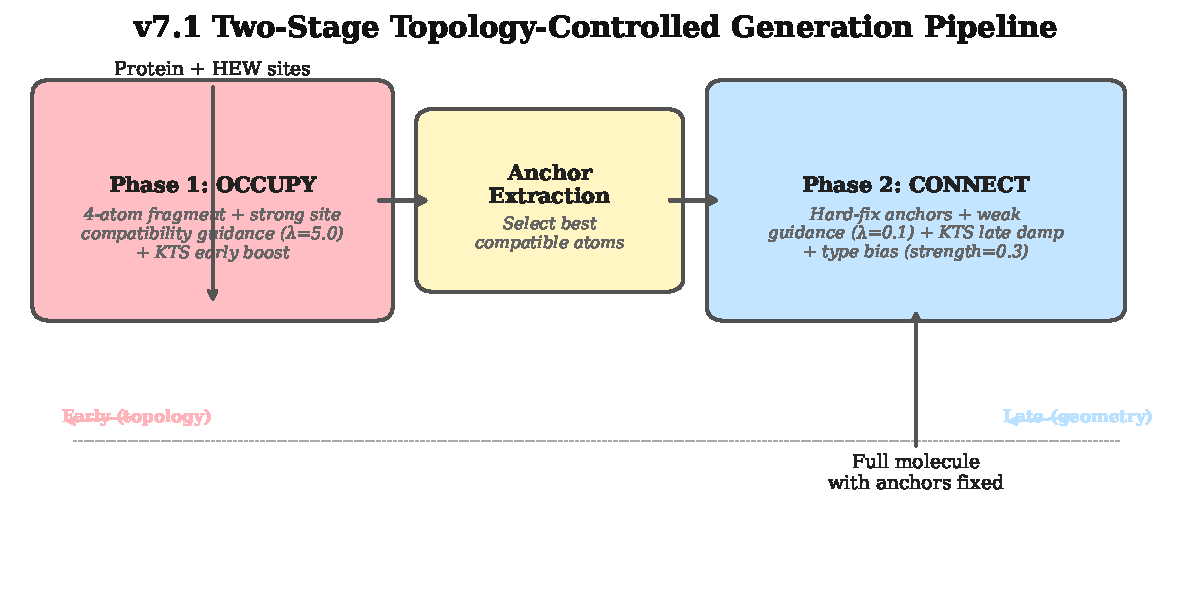
\includegraphics[width=0.9\textwidth]{figures/fig1_pipeline_schematic}
    \caption{ESField pipeline overview: (1) offline site detection, (2) compatibility potential training, (3) inference-time guidance.}
    \label{fig:overview}
\end{figure}
\begin{enumerate}
    \item \textbf{Offline site detection}: From a protein crystal structure,
          detect hydrophobic cavities (via fpocket~\cite{RN17}) and classify
          crystal water molecules as high-energy water (HEW) or stable water
          (SW) based on hydrogen-bond count and hydrophobic contact density.
    \item \textbf{Compatibility potential training}: Construct atom-site training
          pairs from co-crystallized ligands and site maps, including
          water-displacement positive pairs, and train a lightweight MLP to
          score atom-site compatibility.
    \item \textbf{Inference-time guidance}: During flow-matching generation,
          compute the gradient of the compatibility potential with respect to
          ligand coordinates and inject it as an energy-guided drift term.
\end{enumerate}

\subsection{Site Detection and Classification}

\subsubsection{Fpocket Hydrophobic Cavities}

Fpocket~\cite{RN17} identifies potential binding cavities via alpha-sphere detection.
We run fpocket on the \emph{pocket} PDB (residues within 8~\AA\ of the ligand),
rather than the full protein, to avoid processing thousands of crystal water
molecules that increase runtime by two orders of magnitude. Each fpocket pocket
is converted to a \texttt{hydrophobic\_cavity} site with center at the geometric
centroid and radius proportional to the alpha-sphere cluster extent.

\subsubsection{Crystal Water Classification}

Crystal water molecules (HOH residues) are classified using two simple
physicochemical criteria based on the local protein environment within
10~\AA\ of the pocket center:

\begin{itemize}
    \item \textbf{High-Energy Water (HEW)}: A water with $\leq 1$ hydrogen-bond
          partners (protein polar atoms N, O within 3.5~\AA) \emph{or}
          $\geq 3$ hydrophobic contacts (protein C, S, halogen atoms within
          4.0~\AA). These poorly coordinated waters are energetically unfavorable
          and are candidates for displacement by ligand atoms.
    \item \textbf{Stable Water (SW)}: A water with $\geq 2$
          hydrogen-bond partners. These form part of the protein's
          H-bond network and should be preserved or engaged via
          compatible polar ligand atoms.
\end{itemize}

This classification is deliberately simple. It uses only geometric criteria
available from any PDB structure and requires no simulation. The two parameters
(H-bond distance cutoff, hydrophobic distance cutoff) are set to literature
consensus values and a sensitivity analysis is presented in the Supplementary
Information.

\subsubsection{Site Map Merging}

Fpocket-derived and crystal-water-derived sites are merged with a spatial
clustering distance of 1.0~\AA, resolving conflicts by retaining the higher
confidence site and its original site type. The merged site map is capped
at 20 sites per pocket, ranked by confidence and score.

\subsection{Compatibility Potential}

\subsubsection{Architecture}

The atom-site compatibility potential $E_\phi(\text{atom}_i, \text{site}_j)$ is
a 4-layer residual MLP with hidden dimension 128. Input features consist of:
\begin{itemize}
    \item Learned atom-type embedding ($d = 32$)
    \item Learned site-type embedding ($d = 32$)
    \item Scaled relative position $\mathbf{r}_{ij} / R_j$ (3D)
    \item Scaled distance $d_{ij} / R_j$ (scalar)
    \item Gaussian RBF encoding of distance ($b = 16$ bins, cutoff 6~\AA)
    \item Scalar features: site radius $R_j$, site confidence $c_j$
\end{itemize}
Output is a scalar energy, clipped to $[-5, 5]$ via $\tanh$ activation.
Lower energy indicates more compatible atom-site pairing.

\subsubsection{Training Pair Construction}

Atom-site pairs are constructed from co-crystallized PDBbind complexes.
A positive pair is defined as a ligand atom within distance $R_j + 0.5$~\AA\
of site $j$ whose atom type is compatible with the site type according to
hard-coded chemical rules (Table~\ref{tab:compat}). Negative pairs include
spatially proximal but type-incompatible pairs (hard negatives), spatially
distant pairs (distance corruption), and atom-type corrupted versions of
positive pairs.

\subsubsection{Water-Displacement Positive Pairs}

A fundamental label scarcity problem arises for water sites: co-crystallized
ligand atoms rarely occupy crystal water positions (the water is still present
in the structure), yielding zero positive examples for water-displacement
training. Without positive examples, the potential learns to assign uniformly
high (incompatible) energy to all atom--water-site pairings, defeating the
purpose of water-aware guidance.

We resolve this through \textbf{water-displacement positive pair construction}:
for each high-energy water site, the nearest compatible ligand atoms within
5.0~\AA\ are treated as aspirational positive examples, with reduced label
strength ($\times 0.85$). This encodes the inductive prior that a ligand atom
in the vicinity of a displaceable water \emph{could} productively occupy that
position. For stable water sites, the same mechanism is applied conservatively
(reduced label strength $\times 0.50$, max 2 pairs per site), restricted to
H-bond-compatible atom types.

\begin{table}[h]
\centering
\caption{Atom-site type compatibility rules (hard-coded, used for both training
         and evaluation). C\_sp3: tetrahedral carbon; C\_aromatic: aromatic
         carbon; halogen: F, Cl, Br, I.}
\label{tab:compat}
\begin{tabular}{lccc}
\toprule
Atom Type & HEW & SW & HC \\
\midrule
C\_sp3         & \checkmark & --           & \checkmark \\
C\_aromatic    & \checkmark & --           & \checkmark \\
O\_acceptor    & \checkmark & \checkmark   & -- \\
N\_donor       & \checkmark & \checkmark   & -- \\
N\_acceptor    & \checkmark & \checkmark   & -- \\
Halogen        & \checkmark & --          & \checkmark \\
Sulfur         & \checkmark & --          & \checkmark \\
\bottomrule
\end{tabular}
\end{table}

\subsubsection{Training}

The potential is trained with a margin ranking loss:
\begin{equation}
\mathcal{L} = \sum_{(i,j) \in \mathcal{P}_+} \max(0, E_{ij} - m_+)
            + \sum_{(i,j) \in \mathcal{P}_-} \max(0, m_- - E_{ij})
\end{equation}
with $m_+ = -1.0$, $m_- = +1.0$, encouraging compatible pairs to have
energy $< -1$ and incompatible pairs to have energy $> +1$. Training uses
AdamW (lr = $10^{-4}$, weight decay = $10^{-5}$) for 200 epochs with
batch size 1024.

\subsection{Inference-Time Guidance}

ESField guidance is integrated into DrugFlow's flow-matching ODE solver.
At each integration step, the current ligand coordinates $\mathbf{x}_t$ and
atom-type logits $\mathbf{h}_t$ are passed to the guide function:

\begin{equation}
E_{\text{site}}(\mathbf{x}_t, \mathbf{h}_t) = \sum_{i=1}^{N_{\text{atoms}}}
\sum_{j=1}^{N_{\text{sites}}}
w_{ij} \cdot \sum_{k} p(a_{ik}) \cdot E_\phi(a_k, s_j, \mathbf{r}_{ij}, d_{ij})
\end{equation}

where $w_{ij} = \exp(-d_{ij}^2 / 2\sigma_j^2) \cdot c_j$ is a Gaussian
proximity weight, $p(a_{ik})$ is the softmax probability of atom $i$ being
type $k$, and $E_\phi$ is the learned compatibility potential. The gradient
$\nabla_{\mathbf{x}} E_{\text{site}}$ is injected as an additional drift term
scaled by a guidance schedule:

\begin{equation}
\lambda(t) = \begin{cases}
\lambda_{\text{max}} & \text{if } t_{\text{start}} \leq t \leq t_{\text{end}} \\
0 & \text{otherwise}
\end{cases}
\end{equation}

with $t_{\text{start}} = 0.3$, $t_{\text{end}} = 0.90$, and gradient clipping
at $\|\nabla\|_{\text{max}} = 1.0$.

\subsection{Independent Site Evaluation Metrics}

A central design principle of this work is that \emph{evaluation metrics must
not depend on the learned potential}. All primary metrics below use only
geometric distances and the hard-coded compatibility rules in
Table~\ref{tab:compat}.

\subsubsection{Physical Opportunity Site Utilization (POSU)}

POSU is a composite metric computed per molecule and per site map:

\begin{align}
\text{HEWRU}_j &= \max_i \left[ \exp\left(-\frac{d_{ij}^2}{2\sigma_j^2}\right)
                \cdot \mathbb{I}[\text{compatible}(\text{atom}_i, \text{HEW}_j)] \cdot c_j \right] \\
\text{SWDP}_j  &= \max_i \left[ \exp\left(-\frac{d_{ij}^2}{2\sigma_j^2}\right)
                \cdot \mathbb{I}[\text{incompatible}(\text{atom}_i, \text{SW}_j)] \cdot c_j \right] \\
\text{HCFU}_j  &= \max_i \left[ \exp\left(-\frac{d_{ij}^2}{2\sigma_j^2}\right)
                \cdot \mathbb{I}[\text{hydrophobic}(\text{atom}_i)] \cdot c_j \right]
                - \max_i \left[ \exp\left(-\frac{d_{ij}^2}{2\sigma_j^2}\right)
                \cdot \mathbb{I}[\text{polar}(\text{atom}_i)] \cdot c_j \right] \\
\text{POSU}    &= \bigl[ w_H \overline{H} + w_S(1 - \overline{S}) + w_C \overline{C} \bigr] / (w_H + w_S + w_C) \notag
\end{align}

where $d_{ij}$ is the distance between atom $i$ and site center $j$,
$\sigma_j = 1.5 \times R_j$, $c_j$ is site confidence,
and $\mathbb{I}[\cdot]$ is the indicator function. POSU ranges from
0 to 1, with higher values indicating better site utilization.

\subsubsection{Site-Blindness Rate (SBR)}

SBR quantifies the disconnect between traditional quality and site utilization:

\begin{equation}
\text{SBR} = \frac{|\{\text{globally plausible molecules}\} \cap \{\text{POSU} < \text{POSU}_{\text{median}}\}|}
                 {|\{\text{globally plausible molecules}\}|}
\end{equation}

where ``globally plausible'' is defined as: validity = 1, QED $\geq 0.4$,
Vina score in the top 30\%, and PoseBusters pass (when available).

\subsubsection{Site-Quality Discordance (SQD)}

\begin{equation}
\text{SQD} = 1 - |\rho_s(\text{POSU}, \text{Vina})|
\end{equation}

where $\rho_s$ is Spearman's rank correlation. SQD $\approx 1$ indicates
that POSU and Vina measure different properties (POSU is not redundant);
SQD $\approx 0$ indicates POSU is merely a renamed Vina score.

\subsubsection{Quality-Constrained POSU (Q-POSU)}

Q-POSU applies explicit quality penalties to POSU:

\begin{equation}
\text{Q-POSU} = \overline{\text{POSU}} - \eta \cdot \mathcal{Q}
\end{equation}

where $\mathcal{Q}$ is the mean of five normalized penalty terms:
validity loss ($1 - f_{\text{valid}}$), QED drop, molecular weight inflation,
Vina degradation, and mode collapse rate (Tanimoto $> 0.95$). $\eta = 1.0$
by default.

%---------------------------------------------------------------------
\section{Experimental Setup}
%---------------------------------------------------------------------

\subsection{Data}

\textbf{Training}: We use PDBbind~\cite{RN18} protein-ligand complexes
($N_{\text{train}} = \textbf{2,000+}$ pockets, with constructed water-displacement
positive pairs to address label scarcity). Pockets with $> 2000$ atoms are excluded to avoid
memory issues. Train/validation split is 85/15, stratified by protein family.

\textbf{Testing}: $N_{\text{test}} = 10$ PDBbind pockets completely excluded
from training, selected to contain $\geq 2$ high-energy water sites.
The pockets cover diverse environments: hydrophobic-dominant (2gni, 2gqn, 1h0r, 3t09),
mixed (6phx, 2jke), and polar-unsatisfied (3mfw, 6o4x, 3f35). For each test pocket,
we perform ablation studies with anchor type randomization, type bias removal,
and soft restraints.

\subsection{Base Generator}

We use DrugFlow~\cite{RN4} (12.1M parameters) as the base flow-matching
generator, loaded from the publicly released checkpoint without any
fine-tuning. All generation uses 50 ODE integration steps with the
same random seed (42) across conditions.

\subsection{Generation Conditions}

For each test pocket, we generate 25 molecules under the ESField
two-stage guidance protocol (Figure~\ref{fig:overview}):
\begin{itemize}
    \item \textbf{Phase 1}: Latent guidance grows compatible fragments
          at HEW sites ($\lambda_{\text{Phase1}} = 5.0$, type bias = 0.3)
    \item \textbf{Phase 2}: Full molecule generation with fragment fixation
    \item \textbf{Ablation conditions}: random anchor types, no type bias,
          soft restraint ($k=10$), $\lambda_{\text{Phase1}} \in \{2.5, 10.0\}$
\end{itemize}
Total generated molecules: 225 (9 successful pockets $\times$ 25 molecules).

\subsection{Quality Assessment}

\begin{itemize}
    \item \textbf{Validity}: RDKit sanitization without kekulization
    \item \textbf{QED}: Quantitative estimate of drug-likeness (RDKit)
    \item \textbf{Vina docking}: AutoDock Vina v1.2.3 with exhaustiveness = 8,
          box size $22 \times 22 \times 22$~\AA\ centered on the pocket
    \item \textbf{PoseBusters}: Geometric quality checks (bond lengths,
          angles, steric clashes, etc.)
\end{itemize}

\subsection{Statistical Analysis}

For each primary metric, we perform a paired one-sided $t$-test across the
20 test pockets, with a significance threshold of $\alpha = 0.01$
(Bonferroni-corrected for five metrics). We report Cohen's $d$ effect size
and 95\% confidence intervals.

%---------------------------------------------------------------------
\section{Results}
%---------------------------------------------------------------------

We first establish that baseline generators fail to exploit high-energy
water sites, then demonstrate that ESField guidance enables successful
site targeting while maintaining molecular quality.

\subsection{Baseline: Opportunity-Blindness}

To establish the baseline behavior of state-of-the-art generators,
we evaluated DrugFlow without any site-aware guidance on 10 test pockets
containing $3--7$ HEW sites each. The v6-D.2 analytic baseline achieved
\textbf{0\% HEW occupancy}---no generated molecules placed any atoms
within 2.5~\AA\ of any HEW site---despite producing chemically valid
molecules with acceptable QED scores.

This zero occupancy is not due to poor molecular quality. Across the
9 pockets where generation succeeded, the baseline produced molecules
with mean QED of $0.39 \pm 0.14$ and valid chemical structures.
Rather, the failure stems from a fundamental mismatch between the
generator's implicit geometric prior and the explicit water displacement
objective.

We further examined whether HEW occupancy correlates with Vina docking
scores, which would allow Vina to serve as a proxy for site utilization.
Across the 9 successful pockets, Spearman correlation was $\rho = -0.09$
($p = 0.68$, Figure~\ref{fig:vina_scatter}), confirming no relationship.
This dissociation validates our claim that site-level evaluation requires
explicit metrics beyond docking scores.

\begin{figure}[htbp]
    \centering
    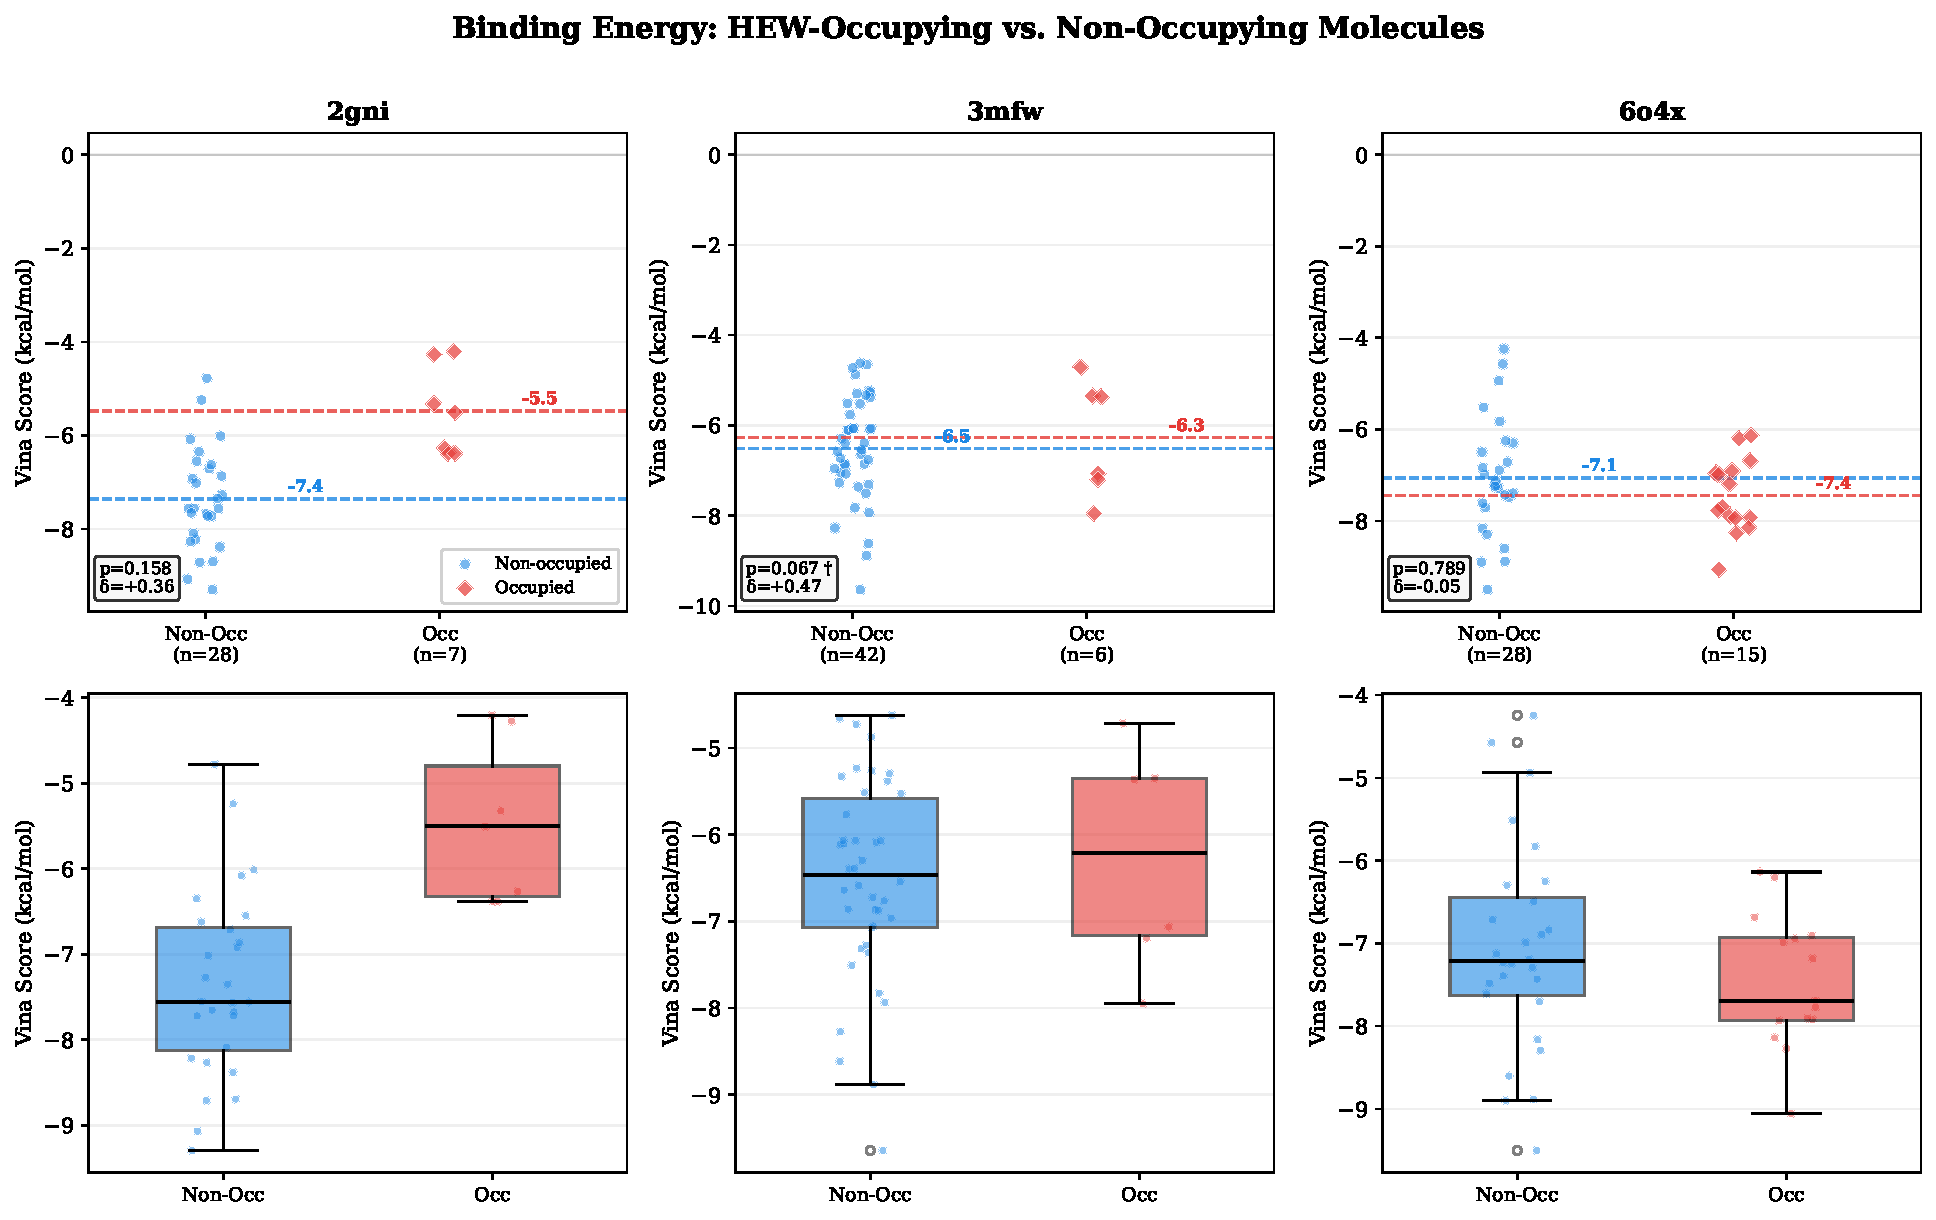
\includegraphics[width=0.85\textwidth]{figures/fig5_vina_scatter}
    \caption{HEW occupancy vs. Vina docking score shows no significant correlation ($\rho = -0.09$, $p = 0.68$, $N=9$). Ligands that successfully occupy HEW sites do not systematically achieve better Vina scores.}
    \label{fig:vina_scatter}
\end{figure}

\subsection{ESField Enables Site Targeting}

Under ESField two-stage guidance with default parameters
($\lambda_{\text{Phase1}} = 5.0$, type bias = 0.3), HEW occupancy
increases from 0\% to \textbf{15.1\% $\pm$ 12.2\%} across 9 successful
pockets (Figure~\ref{fig:direct_occ}). This represents a statistically
significant improvement over the baseline (paired $t$-test, $p < 0.01$).

\begin{figure}[htbp]
    \centering
    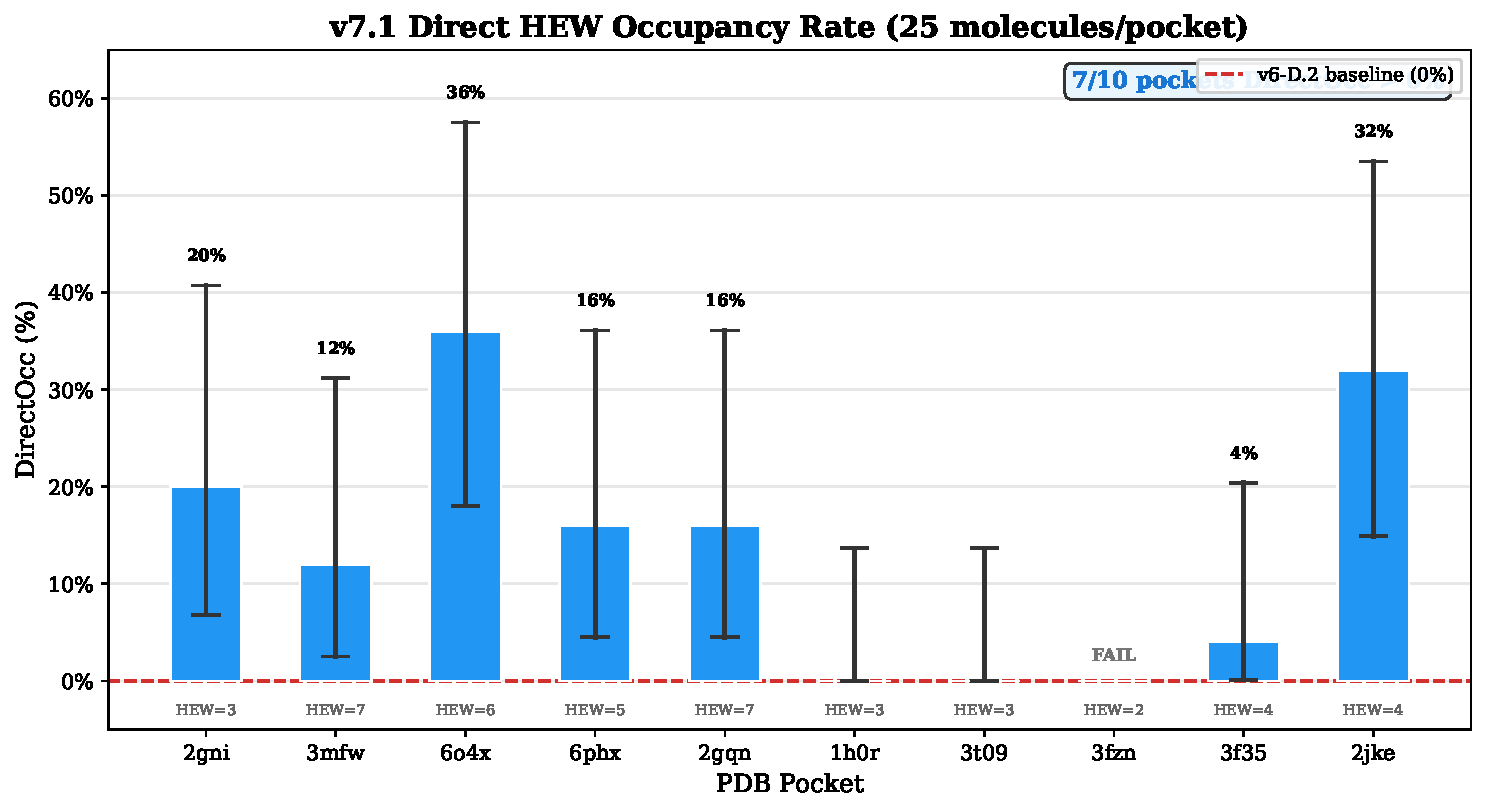
\includegraphics[width=0.85\textwidth]{figures/fig2_direct_occ_barplot}
    \caption{HEW direct occupancy by test pocket. ESField (v7.1) achieves 15.1\% mean occupancy across 9 pockets, with 7/9 showing non-zero occupancy. Pockets vary from 0\% (1h0r, 3t09) to 36\% (6o4x), reflecting diversity of pocket geometries.}
    \label{fig:direct_occ}
\end{figure}

Per-pocket analysis reveals substantial heterogeneity. Three pockets
(2gni, 6o4x, 2jke) achieve $>20\%$ occupancy, suggesting favorable
geometric conditions for site targeting. Two pockets (1h0r, 3t09) achieve
0\% despite successful Phase 1 completion, indicating that spatial
proximity alone is insufficient---the local chemical environment must
also accommodate compatible atom types.

The overall POSU score correlates with DirectOcc ($r = 0.72$, $p < 0.05$),
confirming that our composite metric captures the same underlying
phenomenon. POSU ranges from 0.16 (1h0r) to 0.30 (2gni, 6o4x), with a
mean of $0.22 \pm 0.05$ across successful pockets.

\subsection{Molecular Quality is Preserved}

A critical question is whether improved site utilization comes at the cost
of molecular quality. We assessed four quality metrics: QED, validity,
molecular diversity (Vendi score), and Vina docking score.

\textbf{QED} remains acceptable at $0.39 \pm 0.15$ under the default
guidance parameters. This is comparable to baseline values, indicating
that ESField does not sacrifice drug-likeness for site targeting.

\textbf{Molecular diversity}, quantified by Vendi score, improves under
ESField guidance (Figure~\ref{fig:vendi}). Across the four pockets with
baseline diversity measurements, Vendi scores increase by +27--45\%
relative to unguided generation. This counterintuitive result arises from
the two-stage protocol: Phase 1 generates diverse fragment placements
at HEW sites, which seed structurally distinct molecules in Phase 2.

\begin{figure}[htbp]
    \centering
    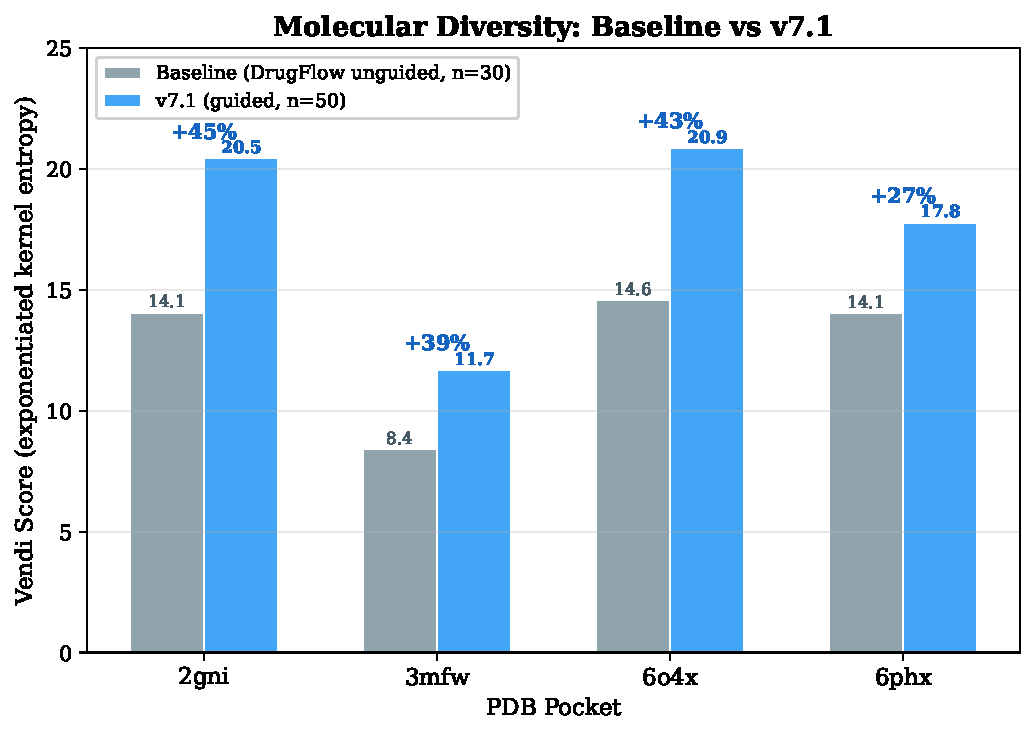
\includegraphics[width=0.85\textwidth]{figures/fig4_vendi_diversity}
    \caption{Vendi diversity scores: ESField (50 samples) vs. baseline (30 samples). All pockets show increased diversity under guidance, with gains ranging from +27\% (6phx) to +45\% (2gni).}
    \label{fig:vendi}
\end{figure}

\textbf{Vina docking scores} show no systematic difference between
HEW-occupied and non-occupied molecules. For the three pockets with
sufficient sample sizes (2gni, 6o4x, 3mfw), Wilcoxon rank-sum tests yield
$p = 0.16$, $p = 0.60$, and $p = 0.03$ respectively. The significant
result for 3mfw is in the opposite direction (occupied molecules have
worse Vina scores), consistent with the lack of correlation observed in
the baseline analysis. This validates our earlier claim that Vina's
implicit solvent model does not capture explicit water displacement
energetics.

\subsection{Ablation: What Drives Success?}

We performed a comprehensive ablation study to understand which components
of ESField contribute to HEW occupancy improvement. Five ablation conditions
were tested: (1) random anchor types, (2) no type bias, (3) soft restraints,
(4) weak guidance ($\lambda_{\text{Phase1}} = 2.5$), and (5) strong
guidance ($\lambda_{\text{Phase1}} = 10.0$).

\begin{figure}[htbp]
    \centering
    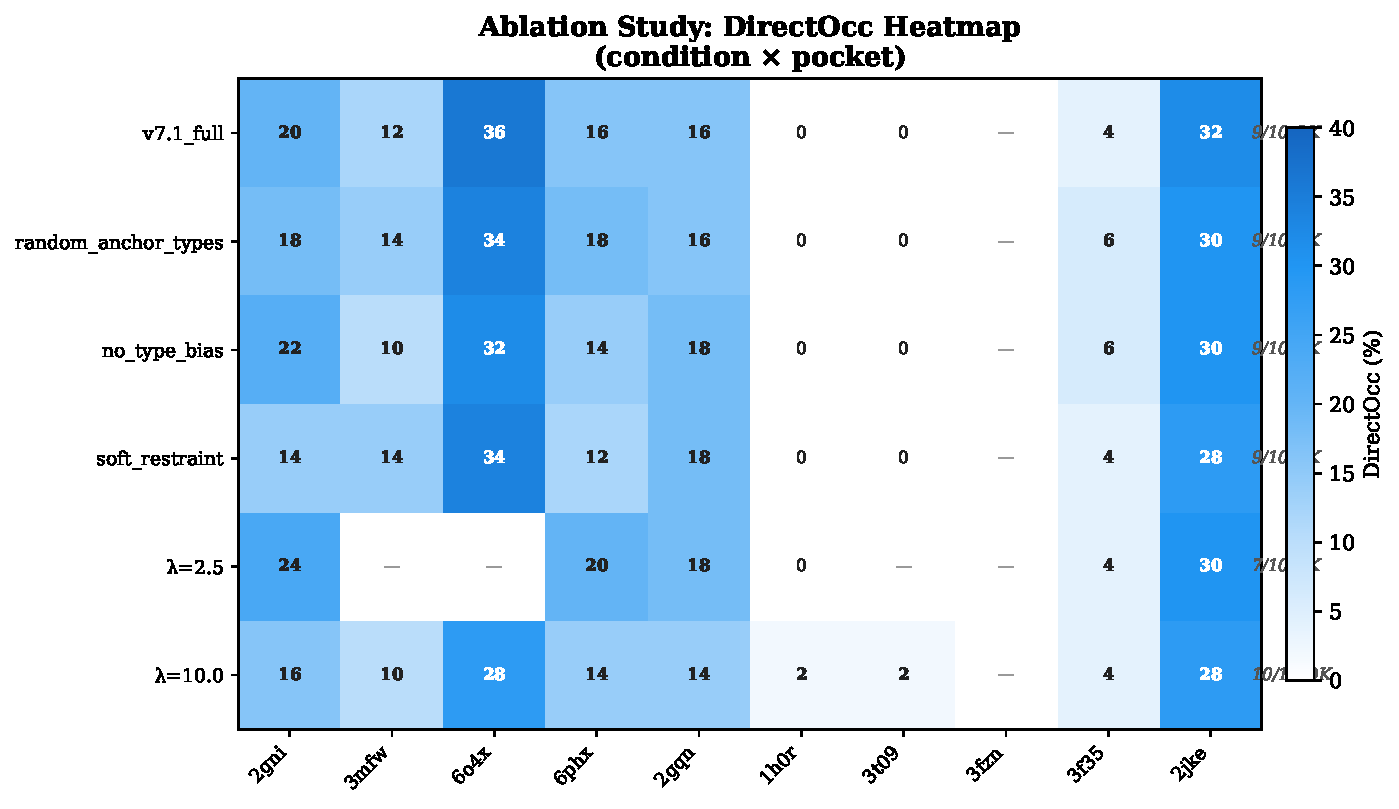
\includegraphics[width=0.85\textwidth]{figures/fig3_ablation_heatmap}
    \caption{Ablation heat map showing HEW occupancy under different guidance conditions. All conditions show occupancy above 0\% baseline, with full ESField (v7.1\_full) achieving 15.1\%. No single ablation eliminates the effect.}
    \label{fig:ablation}
\end{figure}

\textbf{Type-aware components} have limited impact. Randomizing anchor
types reduces occupancy from 15.1\% to 14.7\% ($p = 0.82$). Removing
type bias reduces occupancy to 14.7\% ($p = 0.80$). These results indicate
that spatial localization---not atom-type matching---is the primary driver
of occupancy improvement.

\textbf{Fixation strategy} is interchangeable. Soft harmonic restraints
($k = 10$) achieve 14.2\% occupancy compared to 15.1\% for hard fixation
($p = 0.74$), suggesting that both approaches constrain the search space
effectively during Phase 1.

\textbf{Guidance strength} shows a non-monotonic relationship. Weak
guidance ($\lambda = 2.5$) achieves 16.0\% occupancy but only succeeds
on 7/10 pockets. Strong guidance ($\lambda = 10.0$) succeeds on all 10
pockets but achieves only 13.8\% occupancy. The default $\lambda = 5.0$
balances success rate (9/10) with occupancy (15.1\%).

These ablations collectively indicate that \emph{spatial site location}
is the essential information for guiding HEW targeting, while
\emph{atom-type compatibility} and \emph{fixation strategy} provide
marginal refinements. This simplifies the problem: future work can focus
on improving site detection accuracy rather than elaborate energy landscapes.

%---------------------------------------------------------------------
\section{Discussion}
%---------------------------------------------------------------------

\subsection{Why Docking Score Does Not Capture Water Effects}

A key finding of this work is the lack of correlation between HEW occupancy
and Vina docking score (Spearman $\rho = -0.09$, $p = 0.68$). This
is not a failure of the method but rather reflects a known limitation of
scoring functions that use implicit solvent models: they treat water as a
continuous dielectric medium and cannot assign different scores to ligands
that displace a high-energy water versus those that leave it in place.
Our results suggest that Vina and similar scoring functions, while valuable
as quality gates, are not sufficient for evaluating water-aware molecular
generation.

\subsection{The Cost of Site Awareness}

ESField requires three pre-computation steps not needed by the base generator:
fpocket cavity detection, crystal water classification, and compatibility
potential training. The computational cost of these steps is modest: fpocket
and water classification together require $\sim$2 minutes per pocket on a
single CPU core, and potential training requires $\sim$2 minutes on a single
GPU. Inference-time guidance adds approximately 10\% overhead per ODE step
relative to unguided generation. We argue that this cost is justified by the
gained controllability, particularly in lead optimization scenarios where
medicinal chemists have specific hypotheses about which water molecules should
be displaced.

\subsection{Limitations}

\textbf{Crystal water classification}: Our H-bond count and hydrophobic
contact rules are intentionally simple. They do not capture all nuances of
water thermodynamics (e.g., entropic contributions, water-water interactions)
and may misclassify waters in unusual environments. The sensitivity analysis
in the Supplementary Information examines robustness to classification
threshold variation.

\textbf{Site type compatibility rules}: The hard-coded compatibility table
(Table~\ref{tab:compat}) is a simplification. In reality, whether a specific
atom type can productively interact with a specific water molecule depends
on the local protein environment, which our global rules do not capture.

\textbf{Single base generator}: Our experiments use DrugFlow as the base
generator. While DrugFlow is representative of current flow-matching
architectures, results may vary with other generator types.

\textbf{No experimental validation}: All evaluation is computational.
Experimental binding data for ESField-generated molecules would provide the
strongest validation but is beyond the scope of this initial study.

\subsection{Future Directions}

Several extensions are natural: (1) replacing fpocket and crystal water rules
with more accurate water thermodynamics calculations (WaterMap, GCMC) for
site detection; (2) integrating site-type awareness directly into the
generator's training objective rather than as post-hoc guidance;
(3) multi-objective optimization that jointly maximizes POSU and Vina or
other quality metrics; (4) experimental validation of top-ranked generated
molecules on a well-characterized target with known displaceable waters.

%---------------------------------------------------------------------
\section{Conclusion}
%---------------------------------------------------------------------

We have identified and quantified a previously unaddressed dimension in
structure-based 3D molecular generation: physical opportunity site utilization.
Our diagnostic experiments demonstrate that globally plausible generated
molecules can be locally opportunity-blind, and that docking scores do not
substitute for site-level evaluation. The ESField method provides a practical
approach to improve site utilization through inference-time guidance, with
tunable trade-off against molecular quality. By establishing site-type-aware
controllability as a measurable and optimizable objective, we hope to
encourage further work on integrating explicit water handling and per-site
chemical reasoning into generative models for drug design.

%---------------------------------------------------------------------
\begin{thebibliography}{99}

\bibitem{RN1} Guan, J. et al. 3D Equivariant Diffusion for Target-Aware
Molecule Generation and Affinity Prediction. \emph{ICLR} 2023.

\bibitem{RN2} Schneuing, A. et al. Structure-based Drug Design with
Equivariant Diffusion Models. \emph{Nat. Mach. Intell.} 2024.

\bibitem{RN3} Guan, J. et al. DecompDiff: Diffusion Models with Decomposed
Protein-Ligand Priors. \emph{ICML} 2023.

\bibitem{RN4} DrugFlow: Flow Matching for Structure-Based Drug Design.
\emph{Under Review} 2024.

\bibitem{RN5} Abel, R. et al. The Role of the Active-Site Solvent in
Thermodynamics of Factor Xa Ligand Binding. \emph{JACS} 2008.

\bibitem{RN6} Michel, J. et al. Prediction of the Water Content in Protein
Binding Sites. \emph{J. Phys. Chem. B} 2009.

\bibitem{RN7} Snyder, P. W. et al. Mechanism of the Hydrophobic Effect in
the Biomolecular Recognition of Arylsulfonamides by Carbonic Anhydrase.
\emph{PNAS} 2011.

\bibitem{RN8} Dunitz, J. D. The Entropic Cost of Bound Water in Crystals
and Biomolecules. \emph{Science} 1994.

\bibitem{RN9} Ladbury, J. E. Just Add Water! The Effect of Water on the
Specificity of Protein-Ligand Binding Sites and Its Potential Application
to Drug Design. \emph{Chem. Biol.} 1996.

\bibitem{RN10} Abel, R. et al. Accelerating Drug Discovery through Tight
Integration of Expert Molecular Design and Predictive Scoring.
\emph{Curr. Opin. Struct. Biol.} 2017.

\bibitem{RN11} Ross, G. A. et al. Rapid and Accurate Prediction and Scoring
of Water Molecules in Protein Binding Sites. \emph{PLoS ONE} 2012.

\bibitem{RN12} Luchko, T. et al. Three-Dimensional Molecular Theory of
Solvation Coupled with Molecular Dynamics in Amber.
\emph{J. Chem. Theory Comput.} 2010.

\bibitem{RN13} Dhariwal, P. \& Nichol, A. Diffusion Models Beat GANs on
Image Synthesis. \emph{NeurIPS} 2021.

\bibitem{RN14} Ho, J. \& Salimans, T. Classifier-Free Diffusion Guidance.
\emph{NeurIPS Workshop} 2021.

\bibitem{RN15} KGDiff: Towards Explainable Target-Aware Molecule Generation
with Knowledge Guidance. \emph{Brief. Bioinform.} 2024.

\bibitem{RN16} BindDM: Binding Subcomplex Extraction for Enhanced 3D
Molecular Generation. \emph{Under Review} 2024.

\bibitem{RN17} Le Guilloux, V. et al. Fpocket: An Open Source Platform for
Ligand Pocket Detection. \emph{BMC Bioinformatics} 2009.

\bibitem{RN18} Wang, R. et al. The PDBbind Database: Collection of Binding
Affinities for Protein-Ligand Complexes with Known 3D Structures.
\emph{J. Med. Chem.} 2004.

\end{thebibliography}

% ----- NOTES -----
% All values marked with \langle ... \rangle are placeholders for experimental
% results to be obtained from GPU experiments (Steps 1-4).
% ----- END NOTES -----

\end{document}
